\documentclass[11pt,a4paper]{article}
\usepackage[utf8]{inputenc}
\usepackage[T1]{fontenc}
\usepackage[brazil]{babel}
\usepackage{lmodern}
\usepackage[margin=2cm]{geometry}
\usepackage{amsmath,amssymb}
\usepackage{booktabs}
\usepackage{graphicx}
\usepackage{hyperref}
\usepackage{xcolor}
\usepackage{titlesec}
\usepackage{tabularx}
\usepackage[section]{placeins}
\usepackage{float}

\graphicspath{{../results/figures/}}

\hypersetup{
    colorlinks=true,
    linkcolor=blue!70!black,
    citecolor=blue!70!black,
    urlcolor=blue!70!black
}

\titleformat{\section}{\large\bfseries}{\thesection.}{0.5em}{}
\titleformat{\subsection}{\normalsize\bfseries}{\thesubsection.}{0.5em}{}
\titlespacing*{\section}{0pt}{1.2ex plus 0.5ex minus .2ex}{0.6ex}
\titlespacing*{\subsection}{0pt}{1.0ex plus 0.4ex minus .2ex}{0.4ex}

\setlength{\parskip}{0.45em}
\setlength{\parindent}{0pt}

\begin{document}

\begin{center}
    {\LARGE \textbf{Projeto 2: Aprendizado Não Supervisionado}} \\[0.3em]
    {\large Quantização de Cores com SOM e GNG} \\[0.3em]
    {\large Disciplina: Introdução às Redes Neurais Artificiais} \\[0.3em]
    \textbf{Autor:} Arthur Santos de Oliveira (RA: 156297) \\[0.2em]
    \textbf{Repositório / Código Reprodutível:} \url{https://github.com/Arthur-so/introducao-a-redes-neurais}
\end{center}
\vspace{-0.5em}
\hrule
\vspace{0.8em}

\section{Configuração Experimental}

\textbf{Ideia.} Cada pixel é uma amostra com três características (R, G, B) e cada neurônio é uma cor da paleta. Após o treino, cada pixel recebe a cor do seu neurônio vencedor (BMU), e a imagem passa a ter apenas $K$ cores.

\textbf{Imagens e pré-processamento.} Cinco fotos de $200\times200$ pixels (40.000 amostras cada): (1) lago com floresta, (2) crianças com cachorro, (3) cidade à noite, (4) pôr do sol na praia e (5) flores numa porta. O RGB foi normalizado para $[0, 1]$ e \textbf{todos os pixels} foram usados no treino.

\textbf{Redes.} SOM com grids $4\times4$, $8\times8$ e $16\times16$ e GNG com 16, 64 e 256 neurônios, ou seja, paletas de 16, 64 e 256 cores. São \textbf{30 simulações base} (5 imagens $\times$ 6 redes). O SOM usa a biblioteca MiniSom e a GNG foi implementada em Python. A Tabela~\ref{tab:hiper} resume os hiperparâmetros.

\begin{table}[H]
\centering
\small
\caption{Hiperparâmetros das redes base.}
\label{tab:hiper}
\begin{tabularx}{\textwidth}{lX}
\toprule
\textbf{Item} & \textbf{Valor} \\
\midrule
GNG (valores mais utilizados) & $\eta_b = 10^{-2}$, $\eta_n = 10^{-4}$, $\beta = 0{,}005$, $\alpha = 0{,}5$, $\lambda = 50$, $a_{max} = 90$ \\
SOM & vizinhança gaussiana, $\sigma_0 = 2$, $\eta_0 = 0{,}1$ \\
Decaimento no SOM & padrão do MiniSom: $\eta(t) = \eta_0 / (1 + 2t/T)$, e o mesmo para $\sigma$ \\
Treino & 5 passagens por todos os pixels, em ordem aleatória (igual para SOM e GNG) \\
Inicialização & SOM e GNG começam com as cores de pixels sorteados da imagem \\
Parada da GNG & insere neurônios até o número alvo; depois só adapta, até o fim das 5 passagens \\
Semente & 42 \\
\bottomrule
\end{tabularx}
\end{table}

Os valores do SOM foram escolhidos com um teste nas imagens 1 e 4, com $\sigma_0 \in \{1, 2, 4\}$ e $\eta_0 \in \{0{,}1;\ 0{,}5\}$: $\sigma_0 = 2$ deu o melhor equilíbrio entre os dois erros, e as duas taxas ficaram próximas.

\textbf{Métricas:} foram usados o erro de quantização e o erro topológico.
\begin{itemize}
    \item \textbf{Erro de quantização}: $EQ = \frac{1}{n}\sum_{i=1}^{n} \|x_i - w_{BMU(x_i)}\|$, a distância média entre cada pixel e a cor do seu BMU (RGB em $[0, 1]$). A distância de cada pixel, isoladamente, é o ``erro do pixel'' usado nos histogramas.
    \item \textbf{Erro topológico}: $ET = \frac{1}{n}\sum_{i=1}^{n} t(x_i)$, em que $t(x) = 0$ se o 1º e o 2º BMU de $x$ são vizinhos e $t(x) = 1$ caso contrário. Ou seja, o ET é a proporção de pixels cujos dois neurônios mais próximos não são vizinhos na rede. No SOM, vizinhos são células adjacentes no grid (incluindo as diagonais); na GNG, são neurônios ligados por uma aresta do grafo final.
\end{itemize}

\section{Resultados das 30 Simulações}

A Tabela~\ref{tab:base} traz o EQ e o ET de todas as simulações base, e a Figura~\ref{fig:todas} mostra as 5 imagens quantizadas pelas 6 redes.

\begin{table}[H]
\centering
\small
\caption{Erro de quantização (EQ) e erro topológico (ET) das 30 simulações base. Menor é melhor.}
\label{tab:base}
\begin{tabular}{lcccccc}
\toprule
\textbf{Imagem} & \textbf{SOM 4$\times$4} & \textbf{SOM 8$\times$8} & \textbf{SOM 16$\times$16} & \textbf{GNG 16} & \textbf{GNG 64} & \textbf{GNG 256} \\
\midrule
\multicolumn{7}{l}{\textit{Erro de quantização (EQ)}} \\
1. Lago/floresta      & 0,0175 & 0,0101 & 0,0062 & 0,0151 & 0,0113 & 0,0075 \\
2. Crianças/cachorro  & 0,0997 & 0,0499 & 0,0272 & 0,0748 & 0,0416 & 0,0272 \\
3. Cidade à noite     & 0,0664 & 0,0382 & 0,0242 & 0,0538 & 0,0372 & 0,0293 \\
4. Pôr do sol         & 0,0405 & 0,0210 & 0,0117 & 0,0338 & 0,0192 & 0,0124 \\
5. Flores/porta       & 0,0579 & 0,0349 & 0,0215 & 0,0501 & 0,0320 & 0,0242 \\
\textbf{Média}        & \textbf{0,0564} & \textbf{0,0308} & \textbf{0,0182} & \textbf{0,0455} & \textbf{0,0283} & \textbf{0,0201} \\
\midrule
\multicolumn{7}{l}{\textit{Erro topológico (ET)}} \\
1. Lago/floresta      & 0,1588 & 0,0461 & 0,1752 & 0,0000 & 0,0002 & 0,0016 \\
2. Crianças/cachorro  & 0,0026 & 0,0242 & 0,0607 & 0,0011 & 0,0062 & 0,0044 \\
3. Cidade à noite     & 0,0547 & 0,0376 & 0,0807 & 0,0000 & 0,0035 & 0,0060 \\
4. Pôr do sol         & 0,0016 & 0,0249 & 0,0265 & 0,0008 & 0,0033 & 0,0027 \\
5. Flores/porta       & 0,0699 & 0,1116 & 0,0638 & 0,0001 & 0,0023 & 0,0051 \\
\textbf{Média}        & \textbf{0,0575} & \textbf{0,0489} & \textbf{0,0814} & \textbf{0,0004} & \textbf{0,0031} & \textbf{0,0040} \\
\bottomrule
\end{tabular}
\end{table}

\begin{figure}[H]
\centering
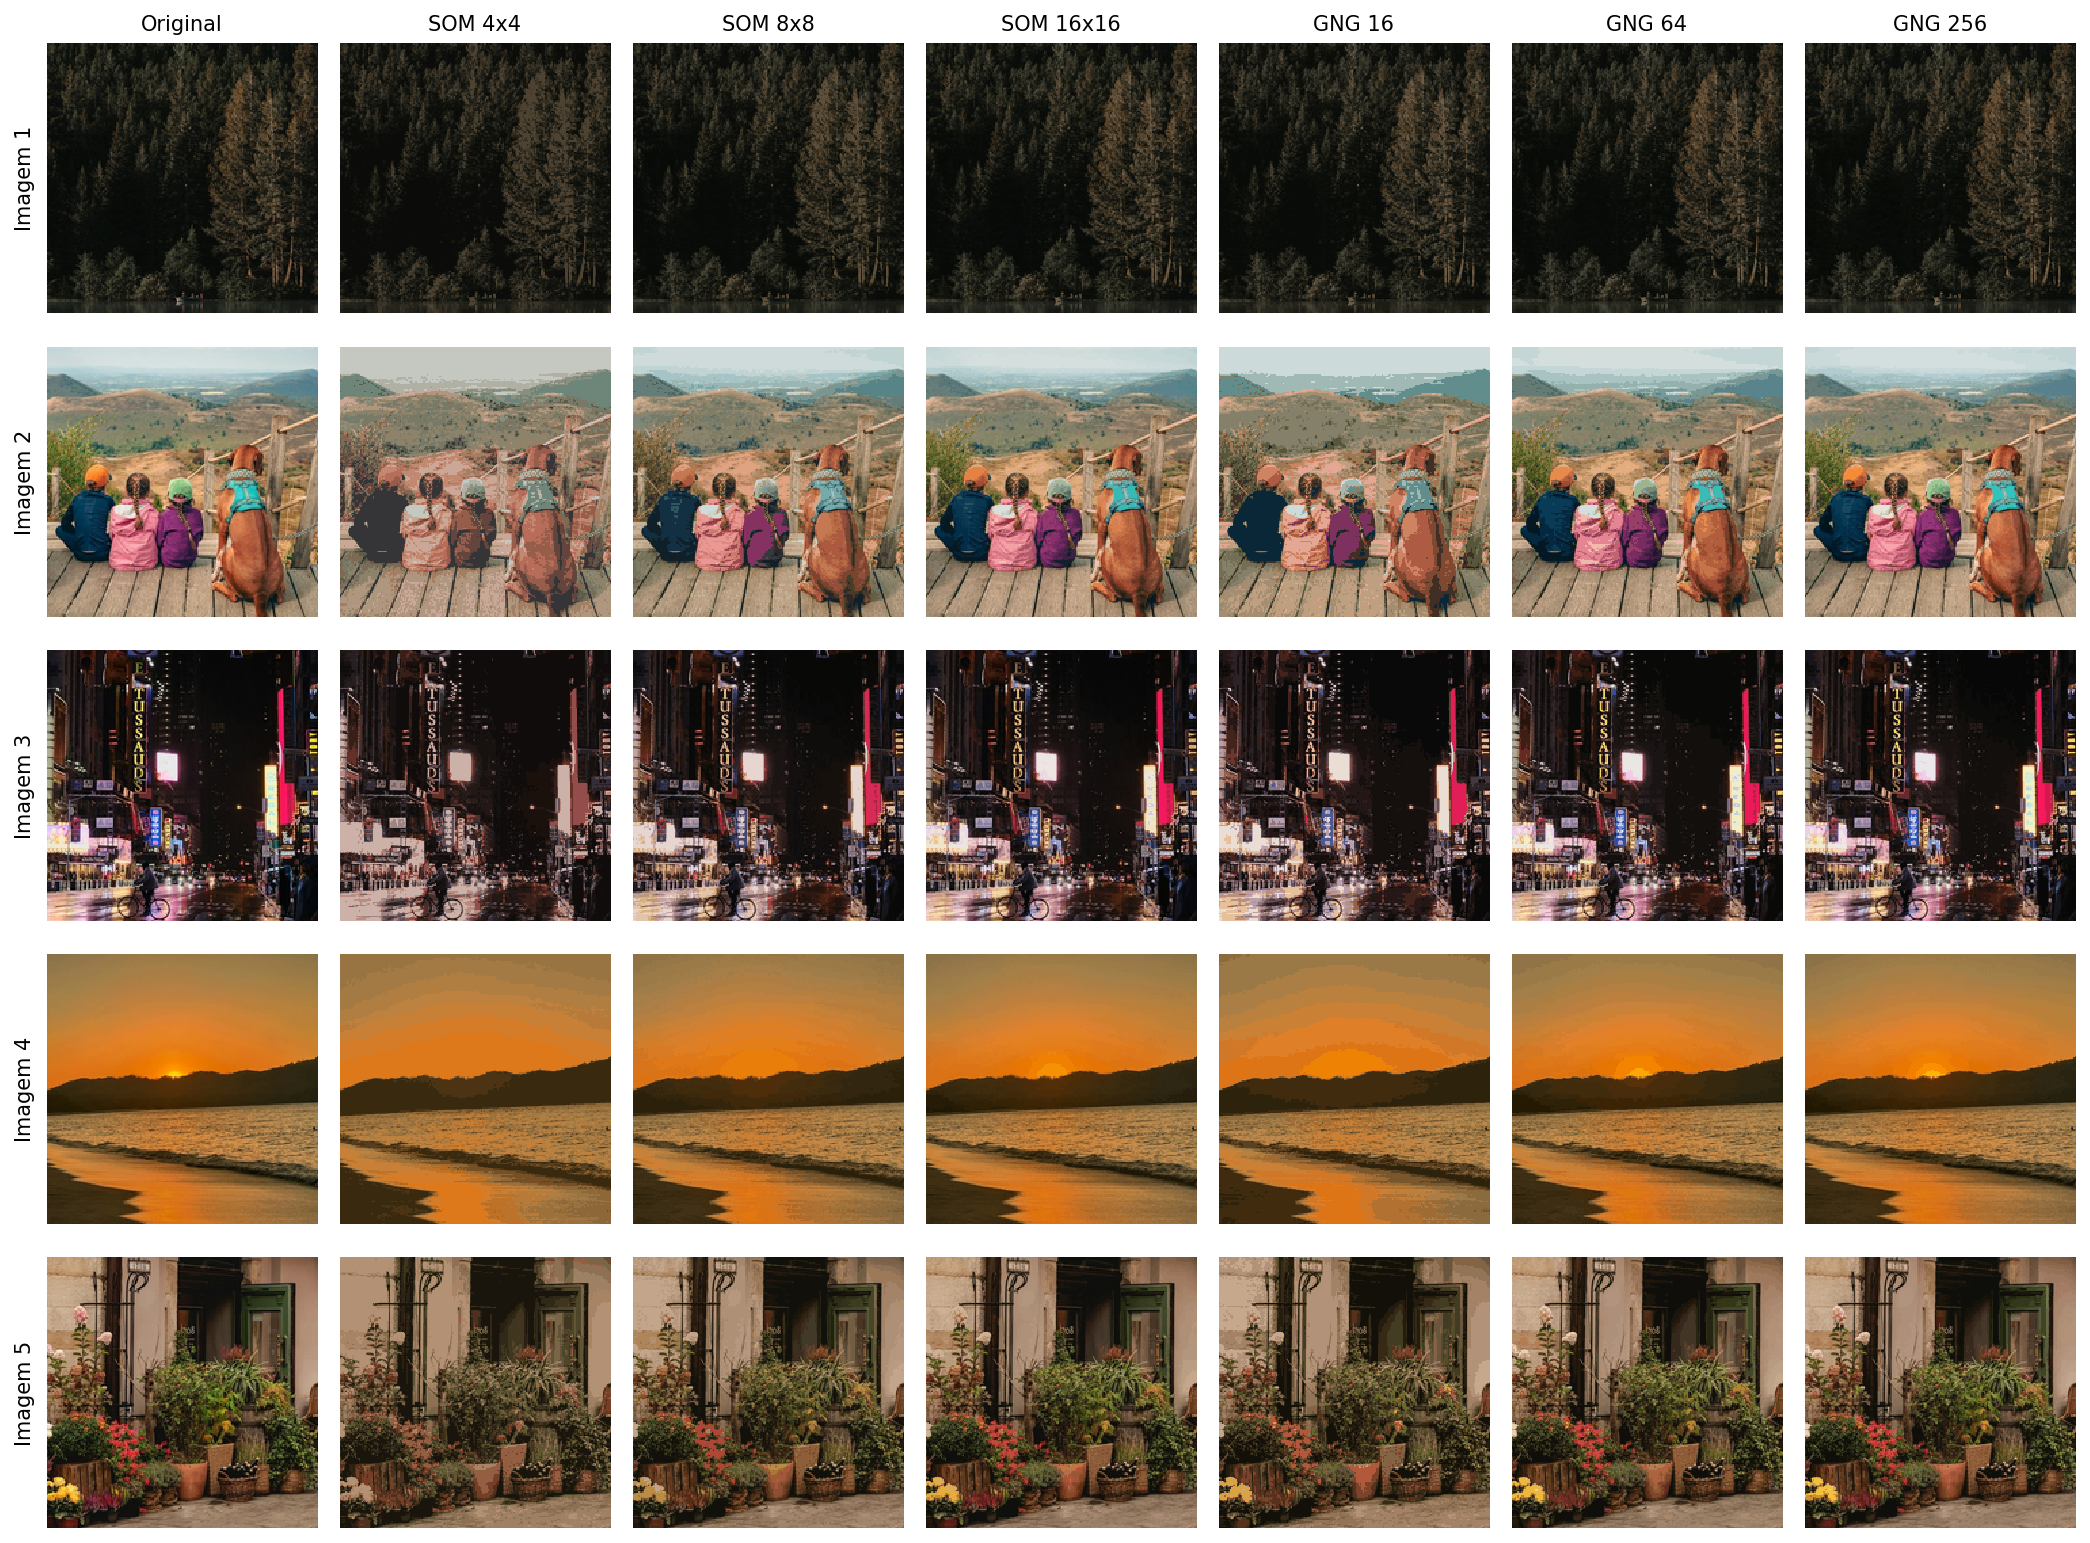
\includegraphics[width=\textwidth]{todas_as_imagens.png}
\caption{As 5 imagens originais (1ª coluna) e quantizadas pelas 6 redes base.}
\label{fig:todas}
\end{figure}

\subsection{Número de cores}

Em todas as imagens e nos dois modelos, \textbf{o EQ cai à medida que o número de cores aumenta}: a cada vez que $K$ é multiplicado por 4, o EQ médio cai entre 29\% e 45\%. Visualmente (Figura~\ref{fig:todas}), com 16 cores todas as imagens continuam reconhecíveis, mas perdem detalhes de cor; com 64 cores as diferenças para o original ficam pequenas; com 256 cores as imagens ficam praticamente iguais ao original.

\subsection{Análise por imagem}

\begin{itemize}
    \item \textbf{Imagem 1 (lago/floresta).} Teve o \textbf{menor EQ} de todas (entre 0,0062 e 0,0175), porque é quase toda verde-escura: as cores ficam próximas umas das outras e poucas cores bastam para representá-la. As seis versões quantizadas são visualmente quase idênticas ao original. Em compensação, foi a imagem com o \textbf{maior ET do SOM} nos grids $4\times4$ (0,1588) e $16\times16$ (0,1752).
    \item \textbf{Imagem 2 (crianças/cachorro).} Teve o \textbf{maior EQ} (0,0997 no SOM $4\times4$), pois reúne muitas cores bem diferentes em áreas pequenas: casacos azul, rosa e roxo, bonés laranja e verde, peitoral azul-turquesa do cachorro. No SOM $4\times4$, o casaco azul fica cinza-escuro, o roxo fica marrom e o céu fica cinza. A GNG 16 mantém o casaco azul-marinho e o roxo. Com 64 cores, quase todas as cores voltam, e o peitoral do cachorro reaparece azul-turquesa na GNG 64.
    \item \textbf{Imagem 3 (cidade à noite).} Mistura um fundo muito escuro com letreiros luminosos. No SOM $4\times4$, o letreiro magenta fica rosa-claro e os letreiros azuis ficam claros e sem cor; a GNG 16 mantém o magenta e o azul. Com 64 cores ou mais, os letreiros ficam fiéis nos dois modelos.
    \item \textbf{Imagem 4 (pôr do sol).} O céu é um degradê suave de laranja, que com 16 cores vira \textbf{faixas} bem visíveis (\textit{banding}); com 64 as faixas ficam discretas. O sol, uma área pequena e mais clara, não aparece no SOM $4\times4$ e só fica amarelo, como no original, no SOM $16\times16$ e na GNG 64 e 256.
    \item \textbf{Imagem 5 (flores/porta).} Foto com muita textura. No SOM $4\times4$, as flores vermelhas ficam salmão-acinzentado e as amarelas ficam quase brancas; a GNG 16 mantém as duas cores. Com 64 cores, as flores ficam fiéis nos dois modelos.
\end{itemize}

\textbf{Padrão comum:} com 16 cores, \textbf{o SOM perde as cores saturadas que ocupam áreas pequenas} (casacos, letreiros, flores) e as troca por tons acinzentados, enquanto a GNG tende a mantê-las. A Figura~\ref{fig:paletas} mostra isso nas paletas da imagem 2: a do SOM $4\times4$ não tem nenhum azul nem roxo.

\begin{figure}[H]
\centering
\begin{minipage}[b]{0.48\textwidth}
    \centering
    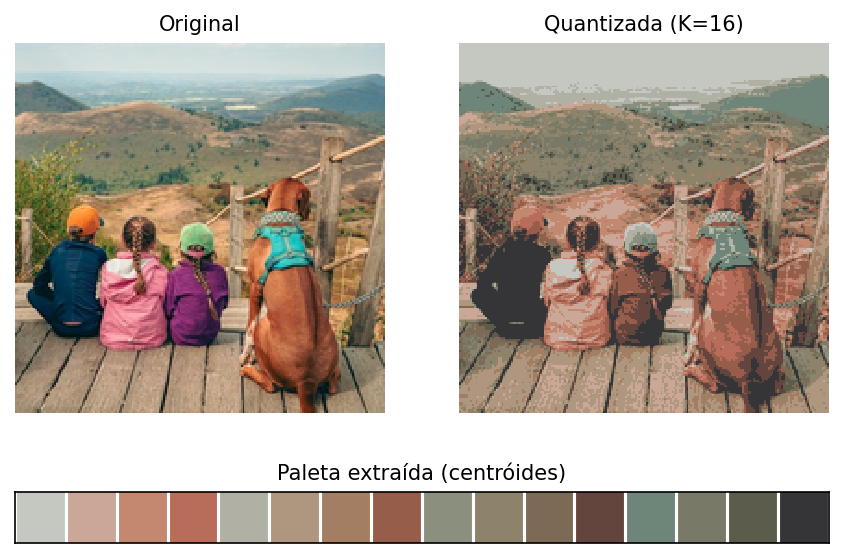
\includegraphics[width=\linewidth]{comparacao_2_criancas_cachorro_SOM_4x4.png}
\end{minipage}
\hfill
\begin{minipage}[b]{0.48\textwidth}
    \centering
    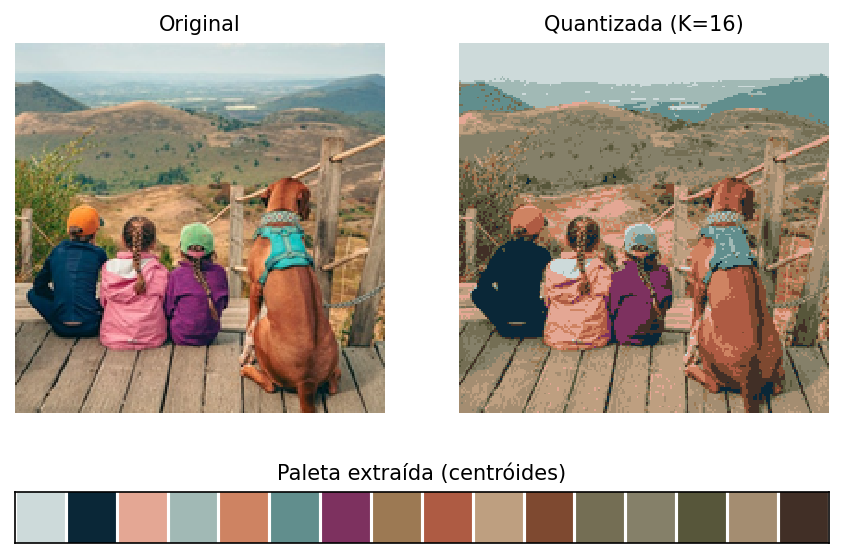
\includegraphics[width=\linewidth]{comparacao_2_criancas_cachorro_GNG_16.png}
\end{minipage}
\caption{Imagem 2 com 16 cores: SOM $4\times4$ (esquerda) e GNG 16 (direita), com a paleta extraída (a cor de cada neurônio) abaixo de cada uma.}
\label{fig:paletas}
\end{figure}

\subsection{SOM vs.\ GNG}
\label{sec:som_gng}

\textbf{Erro de quantização.} Com 16 cores, a \textbf{GNG teve EQ menor nas 5 imagens} (média 0,0455 contra 0,0564 do SOM). Com 64 cores, a GNG venceu em 4 das 5 imagens; a exceção foi a imagem 1. Com 256 cores, o \textbf{SOM $16\times16$ teve o menor EQ} em 4 imagens e empatou na imagem 2.

\textbf{Por quê.} No SOM, cada neurônio puxa também os seus vizinhos do grid, e o mapa inteiro se estica como uma malha sobre as cores. Com poucos neurônios, as cores saturadas de áreas pequenas recebem poucos pixels e acabam sem um neurônio próprio. A GNG insere cada novo neurônio perto do neurônio com \textbf{maior erro acumulado}; pixels de cores mal representadas acumulam erro alto e, por isso, ganham neurônios. Com 256 cores, há neurônios suficientes no SOM para cobrir todas as regiões de cor; já a GNG 256 deixou neurônios sem nenhum pixel (Seção~\ref{sec:hits}), o que reduz o número de cores realmente usadas.

\textbf{Erro topológico.} A GNG teve ET praticamente nulo (no máximo 0,0062); o SOM ficou entre 0,0016 e 0,1752. Esses números \textbf{não devem ser comparados diretamente}. A cada pixel de treino, a GNG cria (ou renova) uma aresta entre os dois neurônios mais próximos desse pixel. Ou seja, a própria regra de treino liga exatamente os pares de neurônios que o ET verifica, e um ET baixo é esperado. No SOM, as vizinhanças são fixadas pelo grid antes do treino, e o ET mostra o quanto as cores da imagem se acomodam a essa malha 2D. O pior caso do SOM foi a imagem 1: com cores muito concentradas, é mais difícil estender o grid sobre elas sem dobras.

\section{Distribuição dos Erros}

A Figura~\ref{fig:hist} mostra o histograma do erro de cada pixel, para as 5 imagens.

\begin{figure}[H]
\centering
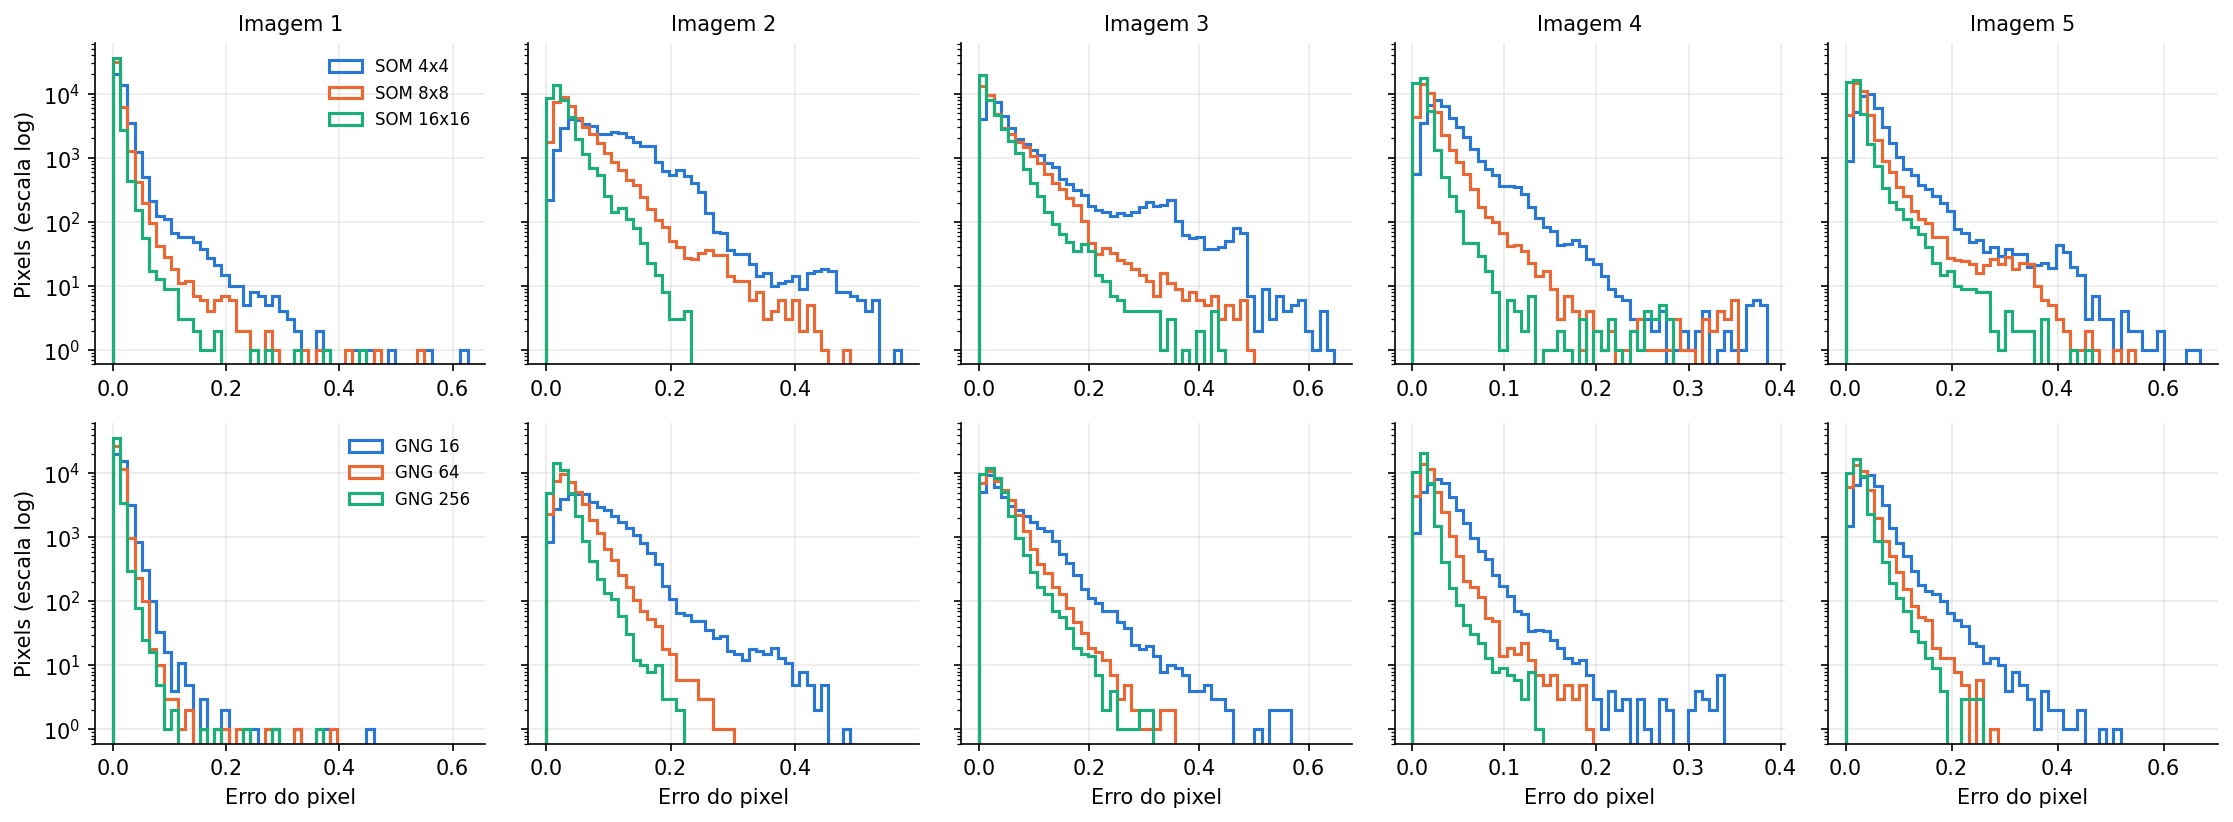
\includegraphics[width=\textwidth]{histogramas.png}
\caption{Histograma do erro por pixel (distância ao BMU) para cada imagem. Linha de cima: SOM; linha de baixo: GNG. O eixo vertical está em escala log.}
\label{fig:hist}
\end{figure}

\begin{itemize}
    \item \textbf{Formato.} Em todas as imagens, a maioria dos pixels tem erro pequeno, mas há uma \textbf{cauda longa}: poucos pixels com erro bem maior que a média. Esses pixels são os de cores raras, que não ganharam um neurônio próprio.
    \item \textbf{Número de cores.} Mais neurônios deslocam a distribuição para a esquerda e encurtam a cauda: com 256 cores, quase não há pixels com erro alto.
    \item \textbf{SOM vs.\ GNG.} Com 16 cores, a cauda do SOM vai até erros maiores que a da GNG em todas as imagens. Nas imagens 2 e 3, o SOM $4\times4$ forma até um segundo ``morro'' de pixels com erro alto, que provavelmente corresponde aos casacos e letreiros saturados que mudaram de cor na Figura~\ref{fig:todas}.
    \item \textbf{Imagem 1.} Tem a distribuição mais concentrada perto de zero, de acordo com o seu EQ, o menor de todos.
\end{itemize}

\textbf{Exemplo de cor rara.} Na imagem 1, uma pessoa num barco é o único detalhe avermelhado, numa imagem quase toda verde-escura. A Tabela~\ref{tab:raro} acompanha o pixel central dessa pessoa, $(185, 100)$, cuja cor é RGB $(129, 90, 81)$, e a Figura~\ref{fig:zoom} mostra a região ampliada.

\begin{table}[htbp]
\centering
\small
\caption{Pixel de cor rara da imagem 1, cor original RGB $(129, 90, 81)$: cor recebida, erro do pixel e número de pixels da imagem que têm o mesmo BMU.}
\label{tab:raro}
\begin{tabular}{lcccc}
\toprule
\textbf{Rede} & \textbf{Cor recebida (RGB)} & \textbf{Erro do pixel} & \textbf{EQ da imagem} & \textbf{Pixels no mesmo BMU} \\
\midrule
SOM 4$\times$4   & (78, 68, 51)   & 0,2482 & 0,0175 & 2312 \\
SOM 8$\times$8   & (95, 81, 59)   & 0,1609 & 0,0101 & 669 \\
SOM 16$\times$16 & (109, 94, 74)  & 0,0840 & 0,0062 & 163 \\
GNG 16           & (109, 92, 71)  & 0,0882 & 0,0151 & 288 \\
GNG 64           & (118, 100, 81) & 0,0601 & 0,0113 & 96 \\
GNG 256          & (123, 105, 86) & 0,0666 & 0,0075 & 60 \\
\bottomrule
\end{tabular}
\end{table}

\begin{figure}[htbp]
\centering
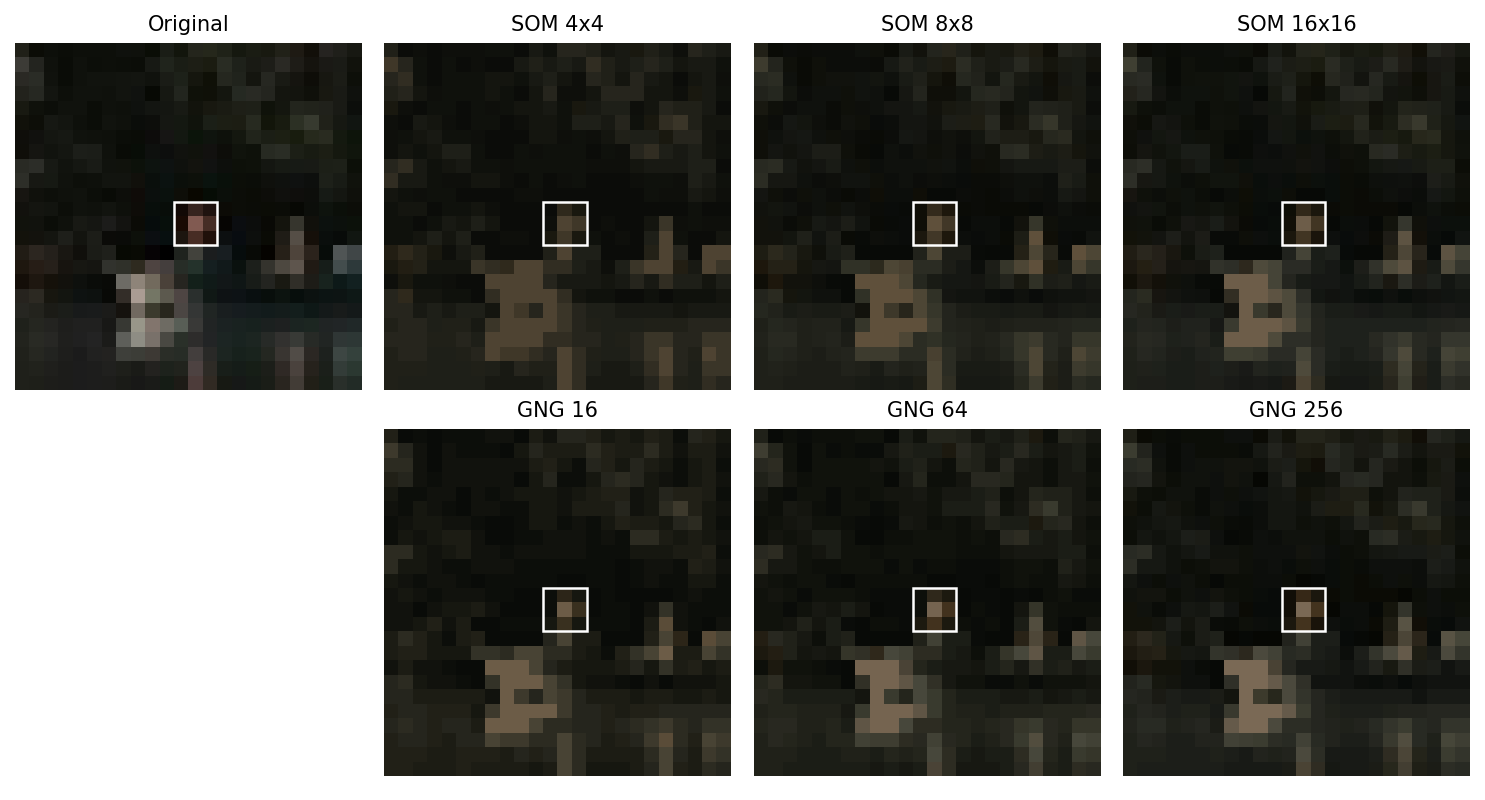
\includegraphics[width=0.6\textwidth]{pixel_raro_zoom.png}
\caption{Região de $24\times24$ pixels em volta do pixel de cor rara (quadrado branco), ampliada.}
\label{fig:zoom}
\end{figure}

\textbf{A cor avermelhada some em todas as redes.} O pixel sempre recebe um marrom ou bege, com erro muitas vezes maior que o EQ da imagem (no SOM $4\times4$, 0,2482 contra 0,0175). Com mais neurônios, a cor recebida se aproxima da original e o BMU passa a ser compartilhado com menos pixels (de 2312 para 60), mas nenhuma rede criou um neurônio avermelhado. \textbf{Por quê:} o detalhe ocupa poucos pixels entre 40.000, e os neurônios se deslocam para onde há muitas amostras.

\section{Uso dos Neurônios (Hit Maps)}
\label{sec:hits}

O \textit{hit map} mostra \textbf{quantos pixels cada neurônio captura}, isto é, para quantos pixels ele é o BMU. A Figura~\ref{fig:hits} mostra os \textit{hit maps} da imagem 2, a mais colorida. Como ler:
\begin{itemize}
    \item \textbf{SOM (linha de cima):} cada célula é um neurônio, na sua posição no grid, pintada com a cor do neurônio; o número é a quantidade de pixels que ele captura.
    \item \textbf{GNG (linha de baixo):} a GNG não tem grid, então cada barra é um neurônio, pintada com a sua cor. As barras estão ordenadas do neurônio mais usado para o menos usado, e a altura (em escala log) é o número de pixels.
\end{itemize}

\begin{figure}[htbp]
\centering
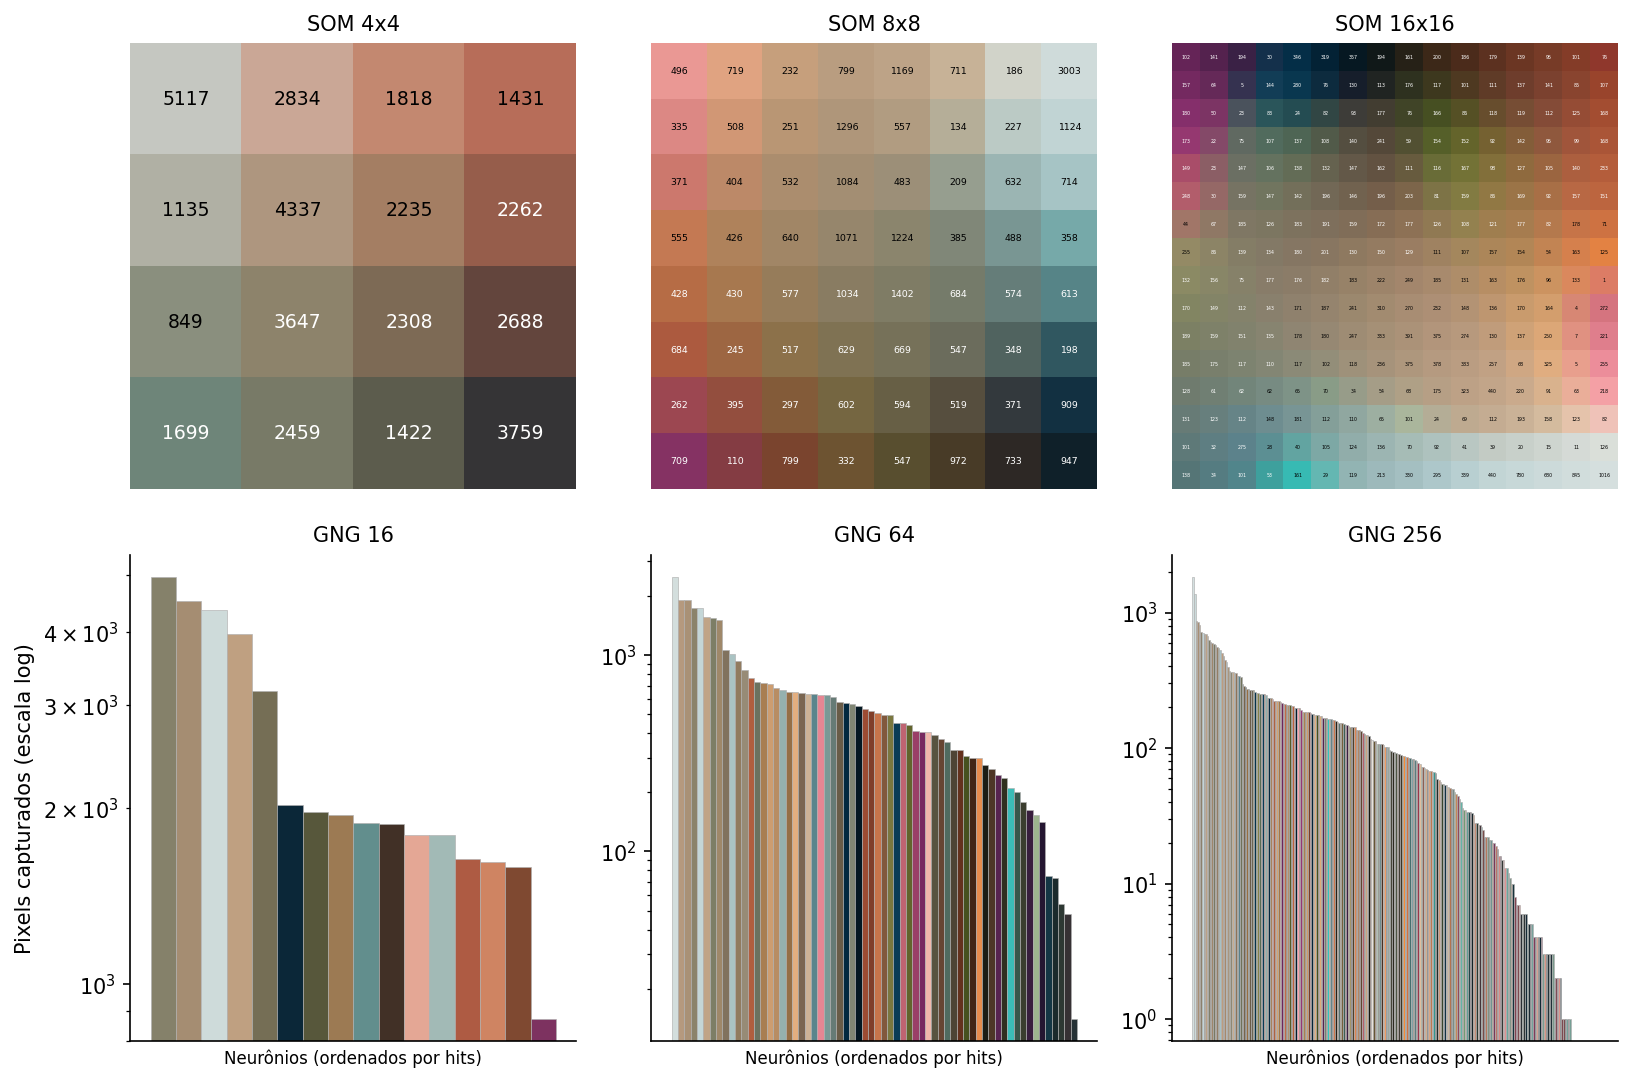
\includegraphics[width=0.85\textwidth]{hit_map_2_criancas_cachorro.png}
\caption{\textit{Hit maps} da imagem 2. SOM: células do grid com a cor do neurônio e o número de pixels capturados. GNG: uma barra por neurônio, ordenadas do mais usado ao menos usado (escala log).}
\label{fig:hits}
\end{figure}

\textbf{O que a figura mostra:}
\begin{itemize}
    \item \textbf{Organização do SOM.} Células vizinhas têm cores parecidas: no grid $4\times4$, os tons claros do céu ficam no canto superior esquerdo, os tons avermelhados (cachorro, casaco rosa) à direita e os escuros no canto inferior direito. A cor muda aos poucos pelo grid, também no $8\times8$ e no $16\times16$. Isso é a preservação topológica, e combina com o ET baixo do SOM nessa imagem (0,0026 no $4\times4$).
    \item \textbf{Cores ausentes no SOM $4\times4$.} Nenhuma das 16 células é azul ou roxa, o que explica por que os casacos mudaram de cor na Figura~\ref{fig:todas}. Na GNG 16, há uma barra azul-marinho e uma roxa (a menor de todas): a GNG reservou neurônios para essas cores, embora sejam pouco frequentes.
    \item \textbf{Distribuição do uso.} No SOM $4\times4$, o neurônio mais usado (cinza-claro, céu) captura 5117 pixels, 12,8\% da imagem. Na GNG 16, o uso fica mais equilibrado, e o neurônio roxo é o menos usado. Na GNG 256, o uso cai de forma contínua da esquerda para a direita, e o espaço vazio à direita das barras corresponde a \textbf{neurônios que não capturam nenhum pixel}.
\end{itemize}

A Tabela~\ref{tab:hits} resume o uso dos neurônios nas 5 imagens.

\begin{table}[htbp]
\centering
\small
\caption{Porcentagem dos pixels capturada pelo neurônio mais usado de cada rede e número de neurônios da GNG 256 sem nenhum pixel. Nas demais redes, todos os neurônios capturam ao menos um pixel.}
\label{tab:hits}
\setlength{\tabcolsep}{4.5pt}
\begin{tabular}{lccccccc}
\toprule
& \multicolumn{6}{c}{\textbf{\% dos pixels no neurônio mais usado}} & \textbf{Sem pixels} \\
\textbf{Imagem} & SOM 4$\times$4 & SOM 8$\times$8 & SOM 16$\times$16 & GNG 16 & GNG 64 & GNG 256 & GNG 256 \\
\midrule
1. Lago/floresta     & 24,4 & 7,7 & 3,4 & 17,3 & 12,1 & 4,9 & 52 \\
2. Crianças/cachorro & 12,8 & 7,5 & 2,5 & 12,4 & 6,3 & 4,6 & 17 \\
3. Cidade à noite    & 29,4 & 9,1 & 2,9 & 21,9 & 19,3 & 12,6 & 46 \\
4. Pôr do sol        & 16,8 & 3,4 & 0,9 & 12,3 & 5,8 & 3,1 & 29 \\
5. Flores/porta      & 16,9 & 9,0 & 2,5 & 12,7 & 9,2 & 6,9 & 27 \\
\bottomrule
\end{tabular}
\end{table}

\begin{itemize}
    \item \textbf{Imagens escuras concentram pixels num só neurônio.} Nas imagens 1 e 3, o neurônio mais usado do SOM $4\times4$ (uma cor quase preta) captura 24,4\% e 29,4\% dos pixels: o fundo escuro ocupa boa parte dessas imagens.
    \item \textbf{Com 256 cores, a GNG concentra mais pixels no neurônio mais usado que o SOM}, em todas as imagens (na imagem 3, 12,6\% contra 2,9\%); com 64 cores, isso ocorre em 4 das 5 imagens. Uma explicação provável é que a GNG insere neurônios onde o erro acumulado é maior, e uma região grande e uniforme, como o céu noturno, acumula pouco erro e pode ficar com um único neurônio.
    \item \textbf{Neurônios sem uso na GNG 256.} Em todas as imagens, entre 17 e 52 neurônios da GNG 256 não capturam nenhum pixel, enquanto o SOM usa todos os neurônios. Uma explicação provável é que cada neurônio novo da GNG nasce no ponto médio entre dois neurônios, e esse ponto pode cair numa região de cor sem pixels. Isso ajuda a explicar por que, com 256 cores, o SOM teve EQ menor.
\end{itemize}

\section{Variações: Vizinhança e Taxas}

As variações foram rodadas nas imagens 1 e 4, mudando um parâmetro por vez em relação à configuração base (Tabela~\ref{tab:variacoes}). Na vizinhança \textbf{bubble}, todos os neurônios a menos de $\sigma$ do vencedor no grid recebem o mesmo ajuste e os demais nenhum. No MiniSom, essa região é um quadrado em volta do vencedor.

\begin{table}[H]
\centering
\footnotesize
\caption{Variações nas imagens 1 e 4 (EQ e ET). A linha ``base'' repete a Tabela~\ref{tab:base}.}
\label{tab:variacoes}
\begin{tabular}{llcccccc}
\toprule
& & \multicolumn{2}{c}{\textbf{SOM 4$\times$4}} & \multicolumn{2}{c}{\textbf{SOM 8$\times$8}} & \multicolumn{2}{c}{\textbf{SOM 16$\times$16}} \\
\textbf{Img.} & \textbf{Variação} & EQ & ET & EQ & ET & EQ & ET \\
\midrule
1 & base (gaussiana, $\sigma_0 = 2$, $\eta_0 = 0{,}1$) & 0,0175 & 0,1588 & 0,0101 & 0,0461 & 0,0062 & 0,1752 \\
1 & bubble & 0,0152 & 0,0231 & 0,0091 & 0,3323 & 0,0057 & 0,3287 \\
1 & $\sigma_0 = 1$ & 0,0152 & 0,1210 & 0,0091 & 0,2199 & 0,0058 & 0,2725 \\
1 & $\sigma_0 = 4$ & 0,0289 & 0,0449 & 0,0123 & 0,2179 & 0,0076 & 0,1196 \\
1 & $\eta_0 = 0{,}01$ & 0,0179 & 0,0859 & 0,0102 & 0,1674 & 0,0065 & 0,1500 \\
1 & $\eta_0 = 0{,}5$ & 0,0192 & 0,0921 & 0,0103 & 0,2581 & 0,0064 & 0,0853 \\
4 & base (gaussiana, $\sigma_0 = 2$, $\eta_0 = 0{,}1$) & 0,0405 & 0,0016 & 0,0210 & 0,0249 & 0,0117 & 0,0265 \\
4 & bubble & 0,0338 & 0,1605 & 0,0185 & 0,1516 & 0,0104 & 0,1658 \\
4 & $\sigma_0 = 1$ & 0,0343 & 0,0431 & 0,0182 & 0,0767 & 0,0104 & 0,1684 \\
4 & $\sigma_0 = 4$ & 0,0818 & 0,0208 & 0,0274 & 0,0190 & 0,0145 & 0,0267 \\
4 & $\eta_0 = 0{,}01$ & 0,0420 & 0,0618 & 0,0210 & 0,0278 & 0,0124 & 0,0750 \\
4 & $\eta_0 = 0{,}5$ & 0,0428 & 0,0054 & 0,0212 & 0,0381 & 0,0117 & 0,0416 \\
\midrule
& & \multicolumn{2}{c}{\textbf{GNG 16}} & \multicolumn{2}{c}{\textbf{GNG 64}} & \multicolumn{2}{c}{\textbf{GNG 256}} \\
\midrule
1 & base & 0,0151 & 0,0000 & 0,0113 & 0,0002 & 0,0075 & 0,0016 \\
1 & $\eta_b = 0{,}005$ & 0,0149 & 0,0000 & 0,0111 & 0,0001 & 0,0084 & 0,0012 \\
1 & $\eta_b = 0{,}05$ & 0,0155 & 0,0006 & 0,0099 & 0,0006 & 0,0064 & 0,0044 \\
1 & $\eta_n = 0{,}001$ & 0,0149 & 0,0000 & 0,0104 & 0,0001 & 0,0075 & 0,0012 \\
1 & $\lambda = 25$ & 0,0150 & 0,0001 & 0,0100 & 0,0007 & 0,0078 & 0,0012 \\
1 & $\lambda = 100$ & 0,0153 & 0,0005 & 0,0118 & 0,0021 & 0,0074 & 0,0019 \\
4 & base & 0,0338 & 0,0008 & 0,0192 & 0,0033 & 0,0124 & 0,0027 \\
4 & $\eta_b = 0{,}005$ & 0,0336 & 0,0000 & 0,0198 & 0,0014 & 0,0134 & 0,0022 \\
4 & $\eta_b = 0{,}05$ & 0,0342 & 0,0000 & 0,0185 & 0,0023 & 0,0115 & 0,0058 \\
4 & $\eta_n = 0{,}001$ & 0,0353 & 0,0001 & 0,0193 & 0,0014 & 0,0119 & 0,0027 \\
4 & $\lambda = 25$ & 0,0338 & 0,0008 & 0,0188 & 0,0017 & 0,0121 & 0,0041 \\
4 & $\lambda = 100$ & 0,0337 & 0,0006 & 0,0189 & 0,0014 & 0,0125 & 0,0029 \\
\bottomrule
\end{tabular}
\end{table}

\textbf{Gaussiana vs.\ bubble.} A bubble teve \textbf{EQ menor em todos os casos}, mas \textbf{ET muito maior} em 5 dos 6 (na imagem 4, de 0,0016 para 0,1605 no grid $4\times4$); a exceção foi o grid $4\times4$ da imagem 1. \textbf{Por quê:} na bubble, quando $\sigma$ cai abaixo de 1, só o vencedor aprende, e o mapa para de se organizar mais cedo. Cada neurônio fica livre para se ajustar à sua cor (EQ menor), mas neurônios vizinhos no grid deixam de ter cores parecidas (ET maior). Na gaussiana, os vizinhos continuam recebendo um ajuste menor até o fim, o que mantém o mapa organizado.

\textbf{Raio inicial $\sigma_0$.} $\sigma_0 = 1$ (menos cooperação entre vizinhos) se comporta como a bubble: EQ menor em todos os casos e ET maior em 5 dos 6. $\sigma_0 = 4$ (mais cooperação) aumentou o EQ em todos os casos (na imagem 4, grid $4\times4$, de 0,0405 para 0,0818), mas não reduziu o ET de forma consistente. \textbf{Há uma troca entre EQ e ET}: menos cooperação dá cores mais precisas e um mapa menos organizado; $\sigma_0 = 2$ ficou no meio-termo.

\textbf{Taxa de aprendizado do SOM ($\eta_0$).} A taxa base, 0,1, teve EQ igual ou menor que 0,01 e 0,5 em todos os casos, mas as diferenças são pequenas (a maior foi no grid $4\times4$ da imagem 4: 0,0405 contra 0,0428 com $\eta_0 = 0{,}5$). O ET do SOM mudou bastante entre as taxas, sem uma direção clara.

\textbf{Taxas e $\lambda$ da GNG.} Com $\eta_b = 0{,}05$ (o vencedor se move mais), o EQ caiu nas redes de 64 e 256 neurônios (imagem 1, GNG 256: de 0,0075 para 0,0064), e o ET aumentou em 3 desses 4 casos. Com $\eta_b = 0{,}005$, o EQ da GNG 256 piorou nas duas imagens. A taxa dos vizinhos $\eta_n = 0{,}001$ e as mudanças de $\lambda$ alteraram pouco o EQ e sem direção consistente: com 5 passagens pelos dados, a rede atinge o número alvo de neurônios em qualquer caso e depois só se adapta. \textbf{Os valores base da GNG funcionaram bem} e não precisaram de ajuste.

\section{Discussão e Conclusões}

\begin{itemize}
    \item \textbf{SOM (rede fixa) vs.\ GNG (topologia adaptativa).} Com poucas cores, a GNG representa melhor as imagens, porque coloca neurônios onde o erro é grande e mantém as cores saturadas de áreas pequenas, que o SOM $4\times4$ perde. Com 256 cores, o SOM $16\times16$ fica um pouco à frente, em parte porque alguns neurônios da GNG 256 ficam sem uso. O SOM, por sua vez, organiza as cores no grid de forma que neurônios vizinhos tenham cores parecidas, como se vê nos \textit{hit maps}.
    \item \textbf{Número de cores.} 16 cores bastam para reconhecer as imagens, mas criam faixas nos degradês (imagem 4) e trocam as cores de detalhes (imagens 2, 3 e 5). Com 64 cores o resultado já é bom, e com 256 fica praticamente igual ao original.
    \item \textbf{Cores raras desaparecem.} Detalhes de cor muito pouco frequentes, como a pessoa avermelhada da imagem 1, não ganham um neurônio próprio em nenhuma rede.
    \item \textbf{Vizinhança e taxas.} A vizinhança gaussiana preserva melhor a topologia que a bubble, ao custo de um EQ um pouco maior. As taxas de aprendizado tiveram efeito pequeno no EQ dentro dos valores testados.
\end{itemize}

\end{document}
